\section{Models Shared by Both Analyses}\label{sec:models}
This section gives every equation used by the code. The MTPA problem and the two loss functions are identical in both analyses.

\subsection{Machine and base values}\label{sec:design}
The machine is specified by its base power $P_\mathrm{b}$, base speed $n_\mathrm{b}$ (rpm), DC voltage $V_\mathrm{dc}$, pole pairs $p$ and the per-unit parameters $r_\mathrm{s}$, $l_\mathrm{d}$, $l_\mathrm{q}$. \code{model.design} derives
\begin{align}
V_\mathrm{b}&=\tfrac12 V_\mathrm{dc}, & V_\mathrm{max}&=\tfrac{2}{\sqrt3}V_\mathrm{b}=\tfrac{V_\mathrm{dc}}{\sqrt3}, & \omega_\mathrm{b}&=\tfrac{2\pi}{60}n_\mathrm{b}, & T_\mathrm{b}&=\tfrac{P_\mathrm{b}}{\omega_\mathrm{b}}, \label{eq:base1}\\
\psi_\mathrm{f}&=\frac{V_\mathrm{b}}{\omega_\mathrm{b}\,p}, & Z_\mathrm{b}&=\frac{\big(\sqrt{3/2}\,V_\mathrm{b}\big)^2}{P_\mathrm{b}}, & I_\mathrm{b}&=50\left\lceil\frac{1}{50}\,\frac{2P_\mathrm{b}}{3V_\mathrm{b}}\right\rceil, \label{eq:base2}\\
R_\mathrm{s}&=r_\mathrm{s}Z_\mathrm{b}, & L_\mathrm{d}&=\frac{l_\mathrm{d}Z_\mathrm{b}}{\omega_\mathrm{b}p}, & L_\mathrm{q}&=\frac{l_\mathrm{q}Z_\mathrm{b}}{\omega_\mathrm{b}p}, \label{eq:base3}\\
\omega_\mathrm{m,max}&=\frac{V_\mathrm{max}}{p\,(\psi_\mathrm{f}-L_\mathrm{d}I_\mathrm{b})}. \label{eq:wmax}
\end{align}
$V_\mathrm{b}$ is a peak phase voltage and $I_\mathrm{b}$ a peak current (rounded up to a multiple of \SI{50}{\ampere}). The magnet flux is chosen so that the back-EMF at base speed equals $V_\mathrm{b}$, and $Z_\mathrm{b}$ is the line-to-line base impedance, which equals $V_\mathrm{b}/I_\mathrm{b}$ before rounding. \Cref{eq:wmax} is the speed at which the voltage limit is reached with the full current $I_\mathrm{b}$ in the negative d axis, neglecting $R_\mathrm{s}$ and $L_\mathrm{q}$; it sets the upper end of the speed range. The code raises an error if $L_\mathrm{d}I_\mathrm{b}\ge\psi_\mathrm{f}$ (no finite maximum speed). \Cref{tab:machine} lists the derived values of the six applications.

\begin{table}[ht]
\centering
\caption{Machine rating and derived machine data of the six applications ($p=4$, $r_\mathrm{s}=0.01$, $l_\mathrm{d}=0.55$, $l_\mathrm{q}=0.85$ pu for all).}
\label{tab:machine}
\footnotesize
\begin{tabular}{@{}lrrrrrrrrrrr@{}}
\toprule
Application & $P_\mathrm{b}$ & $n_\mathrm{b}$ & $V_\mathrm{dc}$ & $E_\mathrm{b}$ & $T_\mathrm{b}$ & $I_\mathrm{b}$ & $n_\mathrm{max}$ & $\psi_\mathrm{f}$ & $R_\mathrm{s}$ & $L_\mathrm{d}$ & $L_\mathrm{q}$ \\
 & [kW] & [rpm] & [V] & [kWh] & [N\,m] & [A] & [rpm] & [mWb] & [m\si{\ohm}] & [\si{\micro\henry}] & [\si{\micro\henry}] \\
\midrule
Passenger car & 150 & 5000 & 400 & 75 & 286 & 500 & 12830 & 95.5 & 4.00 & 105 & 162 \\
City bus & 350 & 2500 & 700 & 350 & 1337 & 700 & 6833 & 334.2 & 5.25 & 276 & 426 \\
Heavy-duty truck & 550 & 3000 & 700 & 400 & 1751 & 1050 & 7719 & 278.5 & 3.34 & 146 & 226 \\
Off-road machine & 150 & 2000 & 700 & 200 & 716 & 300 & 5466 & 417.8 & 12.25 & 804 & 1243 \\
Marine vessel & 400 & 1800 & 800 & 1000 & 2122 & 700 & 4919 & 530.5 & 6.00 & 438 & 676 \\
Regional train & 600 & 2000 & 800 & 300 & 2865 & 1000 & 5132 & 477.5 & 4.00 & 263 & 406
\\
\bottomrule
\end{tabular}
\end{table}

\subsection{Cell model and battery sizing}\label{sec:sizing}
\paragraph{Cell.} The cell is described by its open-circuit voltage (OCV) $V_\mathrm{cell}(z)$, a table in the SOC $z$ (\cref{tab:ocv} in the appendix; linear interpolation), and a first-order equivalent circuit (series $R_0$, parallel $R_1\parallel C_1$). The parameters follow from nominal values and second-order scaling polynomials in $z$ (\code{model.cell_state}):
\begin{equation}
R_0(z)=R_{0,\mathrm{nom}}\,\pi_\mathrm{r}(z),\quad R_1(z)=R_{1,\mathrm{nom}}\,\pi_\mathrm{r}(z),\quad C_1(z)=C_{1,\mathrm{nom}}\,\pi_\mathrm{c}(z),
\label{eq:cellrc}
\end{equation}
with $\pi_\mathrm{r}(z)=1.3z^2-1.3z+1.3$, $\pi_\mathrm{c}(z)=-1.3z^2+1.3z+1.3$ (defaults for the Samsung PHEV2 \SI{24}{\ampere\hour} cell), $R_{0,\mathrm{nom}}=\SI{1.2}{\milli\ohm}$, $R_{1,\mathrm{nom}}=\SI{0.7}{\milli\ohm}$, and $C_{1,\mathrm{nom}}=1/(2\pi\cdot\SI{250}{\hertz}\cdot R_{1,\mathrm{nom}})$ so that the RC corner is \SI{250}{\hertz}. \Cref{fig:cell} shows the OCV and the parameters.

\begin{figure}[ht]
\centering
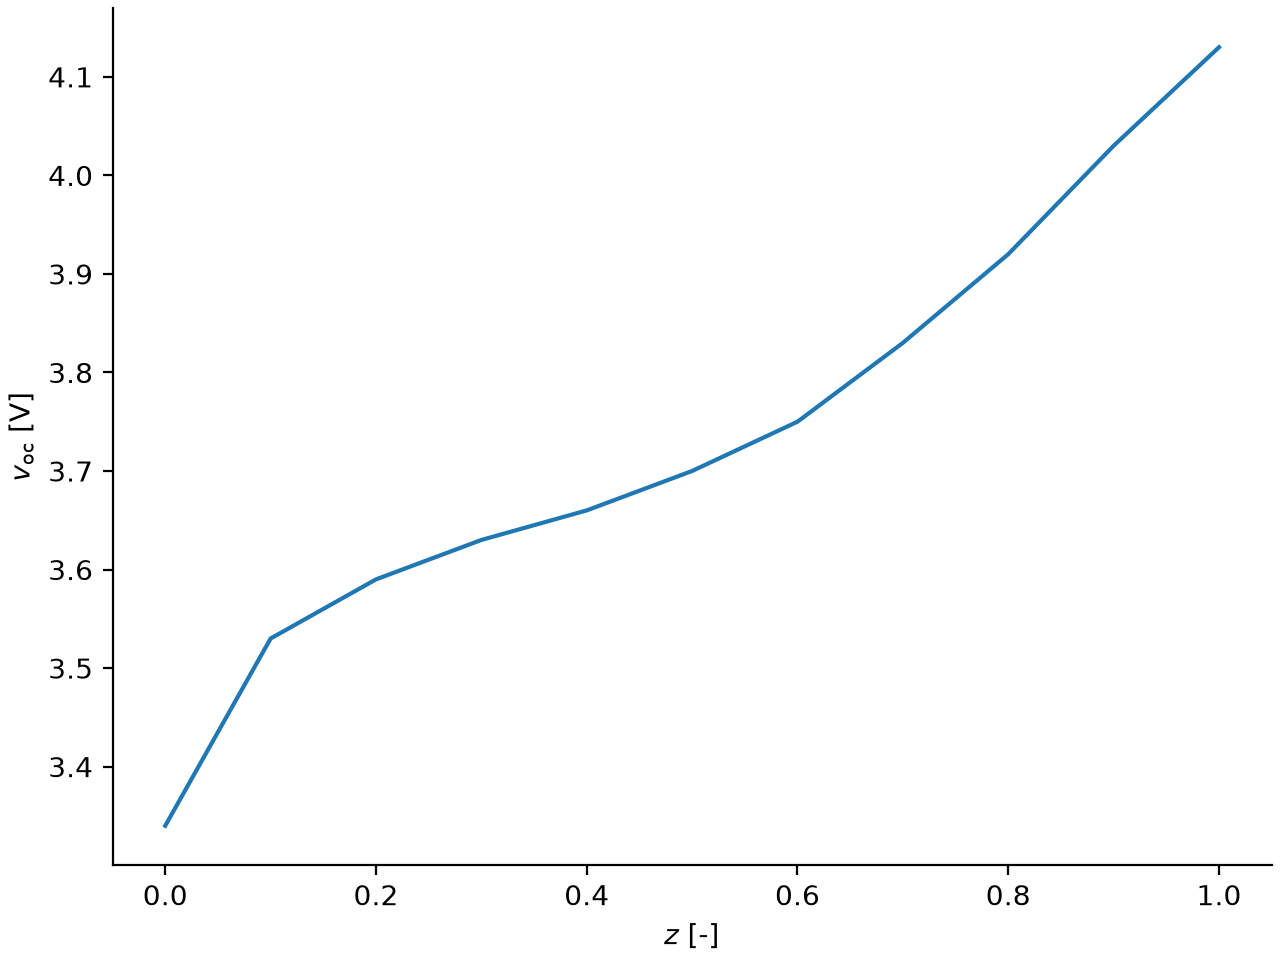
\includegraphics[width=0.48\linewidth]{figures/inputs/battery_ocv.png}\hfill
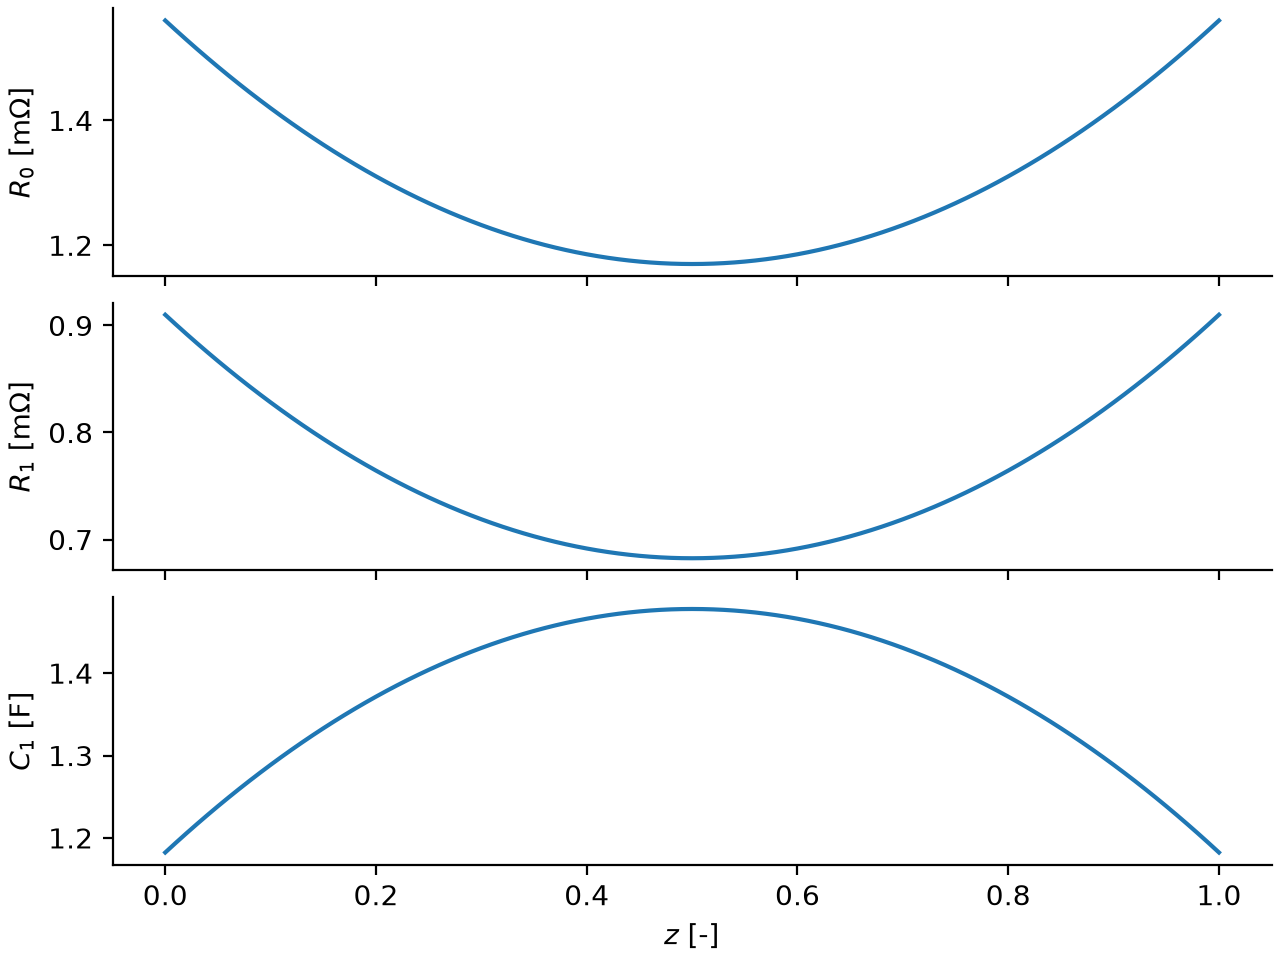
\includegraphics[width=0.48\linewidth]{figures/inputs/battery_parameters.png}
\caption{Cell data of the NMC cell: open-circuit voltage versus SOC (left) and the SOC-scaled equivalent-circuit parameters (right).}
\label{fig:cell}
\end{figure}

\paragraph{Thermal model of the cell.} Cells are cooled from the bottom, insulated on the sides, with the coolant at the ambient temperature. The steady-state cell temperature for a battery loss $P_\mathrm{b}$ shared equally by $n$ cells is
\begin{equation}
T_\mathrm{cell}=T_\mathrm{amb}+\frac{P_\mathrm{b}}{n}R_\mathrm{th,cell},\qquad R_\mathrm{th,cell}=\frac{l_\mathrm{z}}{k_\mathrm{z}A_\mathrm{z}}=\frac{\SI{0.027}{\metre}}{\SI{25}{\watt\per\metre\per\kelvin}\cdot\SI{3.996e-3}{\metre\squared}}=\SI{0.27}{\kelvin\per\watt}.
\label{eq:tcell}
\end{equation}

\paragraph{2L pack.} With $V_\mathrm{nom}=V_\mathrm{cell}(0.5)$,
\begin{equation}
N_\mathrm{s}=\Big\lceil\frac{V_\mathrm{dc}}{V_\mathrm{nom}}\Big\rceil,\qquad N_\mathrm{p}=\Big\lceil\frac{E_\mathrm{b}}{Q_\mathrm{cell}V_\mathrm{nom}N_\mathrm{s}}\Big\rceil.
\label{eq:pack2l}
\end{equation}
The DC-link voltage at the present SOC is $V_\mathrm{dc}(z)=N_\mathrm{s}V_\mathrm{cell}(z)$.

\paragraph{BI-MMC sizing.} The user chooses the number of series cells per submodule, $\Nssm$ (default 10); the number of submodules and parallel cells follow. The BI-MMC phase-voltage amplitude is $\Nsm\Nssm V_\mathrm{cell}(1-r)$, where $r$ is the redundant share of the $\Nsm$ SMs, and it must reach the peak phase voltage $V_\mathrm{max}$ of \cref{eq:base1} at the nominal cell voltage. Rounding up (\code{model.design}),
\begin{equation}
\Nsm=\Big\lceil\frac{V_\mathrm{max}}{V_\mathrm{nom}\,\Nssm\,(1-r)}\Big\rceil,\qquad
\Npsm=\Big\lceil\frac{E_\mathrm{b}}{3\,\Nsm\,\Nssm\,V_\mathrm{nom}\,Q_\mathrm{cell}}\Big\rceil.
\label{eq:npsm}
\end{equation}
The 2L inverter with space-vector modulation reaches $V_\mathrm{dc}/\sqrt3=V_\mathrm{max}$ at the same cell voltage. Because $\Nsm$ and $\Npsm$ are integers, the BI-MMC string voltage is \SIrange{0.7}{4.1}{\percent} above $V_\mathrm{max}$ and the BI-MMC has between $-0.8$ and $+8.4$~\% more cells than the 2L pack (\cref{tab:conv}). Choosing $\Nssm$ per application keeps these deviations small; the passenger car uses $\Nssm=7$ instead of the default, because 10 series cells would give 7 SMs and \SI{20}{\percent} more cells than the 2L pack.

\paragraph{Parallel devices.} The 2L switch needs $N_\mathrm{p,mos}=\lceil I_\mathrm{b}/(\sqrt2 I_\mathrm{rated})\rceil$ devices ($I_\mathrm{rated}=\SI{320}{\ampere}$ RMS). The BI-MMC switch uses $\max\big(\lceil I_\mathrm{b}/(\sqrt2\cdot\SI{400}{\ampere})\rceil,\,4\big)$ devices. \Cref{tab:conv} lists the resulting design of every application.

\begin{table}[ht]
\centering
\caption{Battery and converter design of the six applications (\cref{eq:pack2l,eq:npsm}; cell energy as in \cref{tab:machine}). $N_\mathrm{cells}$ is the total cell count of each drive.}
\label{tab:conv}
\footnotesize
\begin{tabular}{@{}lccccrrr@{}}
\toprule
Application & 2L pack & $N_\mathrm{p,mos}$ (2L) & $\Nsm\times\Nssm$ & $\Npsm$ & $N_\mathrm{p,mos}$ (BI) & $N_\mathrm{cells}$ (2L) & $N_\mathrm{cells}$ (BI) \\
\midrule
Passenger car & $109\mathrm{s}8\mathrm{p}$ & 2 & $9\times7$ & 5.00 & 4 & 872 & 945 \\
City bus & $190\mathrm{s}21\mathrm{p}$ & 2 & $11\times10$ & 12.00 & 4 & 3990 & 3960 \\
Heavy-duty truck & $190\mathrm{s}24\mathrm{p}$ & 3 & $11\times10$ & 14.00 & 4 & 4560 & 4620 \\
Off-road machine & $190\mathrm{s}12\mathrm{p}$ & 1 & $11\times10$ & 7.00 & 4 & 2280 & 2310 \\
Marine vessel & $217\mathrm{s}52\mathrm{p}$ & 2 & $13\times10$ & 29.00 & 4 & 11284 & 11310 \\
Regional train & $217\mathrm{s}16\mathrm{p}$ & 3 & $13\times10$ & 9.00 & 4 & 3472 & 3510
\\
\bottomrule
\end{tabular}
\end{table}

\subsection{MTPA control}\label{sec:mtpa}
In the rotor frame, the stator voltage equations (steady state) and the torque of the PMSM are
\begin{align}
v_\mathrm{d}&=R_\mathrm{s}i_\mathrm{d}-\omega_\mathrm{e}L_\mathrm{q}i_\mathrm{q}, \label{eq:vd}\\
v_\mathrm{q}&=R_\mathrm{s}i_\mathrm{q}+\omega_\mathrm{e}\big(\psi_\mathrm{f}+L_\mathrm{d}i_\mathrm{d}\big), \label{eq:vq}\\
T&=\tfrac32 p\big(\psi_\mathrm{f}i_\mathrm{q}+(L_\mathrm{d}-L_\mathrm{q})i_\mathrm{d}i_\mathrm{q}\big), \label{eq:torque}
\end{align}
with $\omega_\mathrm{e}=p\,\omega_\mathrm{m}$ (\code{model.dq_voltages}). For every operating point $(\omega_\mathrm{m},T^*)$ the code solves the optimisation problem (\code{calc.create_mtpa_optimization_problem})
\begin{equation}
\min_{i_\mathrm{d},i_\mathrm{q}}\; i_\mathrm{d}^2+i_\mathrm{q}^2\quad\text{s.t.}\quad T(i_\mathrm{d},i_\mathrm{q})=T^*,\qquad v_\mathrm{d}^2+v_\mathrm{q}^2< \hat v_\mathrm{max}^2,
\label{eq:mtpa}
\end{equation}
that is, the minimum-current solution that produces the requested torque and respects the voltage limit. It is therefore MTPA below base speed and automatically adds field weakening (negative $i_\mathrm{d}$) when the voltage limit becomes active. The problem is built once with CasADi's \code{Opti} stack, with $T^*$, $\omega_\mathrm{m}$ and $\hat v_\mathrm{max}$ as parameters, and solved with IPOPT (print level 0). Because the torque constraint is bilinear, the problem is non-convex; the previous solution warm-starts the next solve, which in practice keeps the solver on the MTPA branch. After the solve, two checks are applied. A point is marked infeasible (NaN) if IPOPT fails (voltage limit cannot be met), if its power exceeds the rating ($|\omega_\mathrm{m}T^*|>P_\mathrm{b}$, skipped before solving), or if the current exceeds the limit, $i_\mathrm{d}^2+i_\mathrm{q}^2>I_\mathrm{b}^2$. After a failure, the initial guess is reset to zero.

\paragraph{Voltage limit per drive.} The limit $\hat v_\mathrm{max}$ follows the cell OCV at the present SOC and differs between the drives:
\begin{equation}
\hat v_\mathrm{max}^\mathrm{2L}=\frac{N_\mathrm{s}V_\mathrm{cell}(z)}{\sqrt3},\qquad
\hat v_\mathrm{max}^\mathrm{BI}=\Nssm V_\mathrm{cell}(z)\,\Nsm\,(1-r).
\label{eq:vmax}
\end{equation}
The factor $(1-r)$ accounts for the redundant SM share $r$ (default $r=0$). By construction of \cref{eq:npsm}, the BI-MMC limit is equal to or slightly above the 2L limit (by the rounding of $\Nsm$). If both limits are equal, the code solves the MTPA problem once and reuses the currents for both drives.

\subsection{Two-level inverter losses}\label{sec:loss2l}
\code{calc.calc_losses_2l} receives the dq currents and voltages and returns the conduction loss $P_\mathrm{c}$, the switching loss $P_\mathrm{s}$, the battery loss $P_\mathrm{b}$ and the temperatures $\Tj$, $\Tc$.

\paragraph{Conduction loss.} With the stator current amplitude $\Ihat=\sqrt{i_\mathrm{d}^2+i_\mathrm{q}^2}$ and a sinusoidal phase current, each switch conducts half the fundamental period. The RMS current of one device is $\Ihat/(\sqrt2N_\mathrm{p,mos})$, so a device dissipates $\tfrac12\big(\Ihat/(\sqrt2N_\mathrm{p,mos})\big)^2\Rds$ on average, a switch of $N_\mathrm{p,mos}$ devices $\tfrac14\Ihat^2\Rds/N_\mathrm{p,mos}$, and the six switches
\begin{equation}
P_\mathrm{c}^\mathrm{2L}=\frac32\,\Rds\,\frac{i_\mathrm{d}^2+i_\mathrm{q}^2}{N_\mathrm{p,mos}}.
\label{eq:pc2l}
\end{equation}
The model does not distinguish between the transistor and the body diode and ignores the dependence on the modulation index.

\paragraph{Switching loss.} The datasheet gives current- and voltage-slope curves $\mathrm{d}i/\mathrm{d}t$ and $\mathrm{d}v/\mathrm{d}t$ for turn-on and turn-off as functions of the device current (\cref{fig:slopes}); the code interpolates them linearly and holds them constant outside the data range. The average absolute phase current is $\bar\imath=\tfrac{2}{\pi}\Ihat$, the device current $\bar\imath_\mathrm{dev}=\bar\imath/N_\mathrm{p,mos}$, and the four commutation intervals follow from the slopes (slopes in units of per nanosecond):
\begin{equation}
t_\mathrm{ri}=\frac{\bar\imath_\mathrm{dev}}{(\mathrm{d}i/\mathrm{d}t)_\mathrm{on}},\quad
t_\mathrm{fi}=\frac{\bar\imath_\mathrm{dev}}{(\mathrm{d}i/\mathrm{d}t)_\mathrm{off}},\quad
t_\mathrm{rv}=\frac{V_\mathrm{dc}}{(\mathrm{d}v/\mathrm{d}t)_\mathrm{on}},\quad
t_\mathrm{fv}=\frac{V_\mathrm{dc}}{(\mathrm{d}v/\mathrm{d}t)_\mathrm{off}},
\label{eq:times}
\end{equation}
where the slopes are in \si{\ampere\per\nano\second} and \si{\volt\per\nano\second}, so the times are multiplied by $10^{-9}$ to obtain seconds. The slope-based energy per switching event of one switch follows the linear-overlap approach of \cite{graovac2006},
\begin{equation}
E_\mathrm{sw}=\tfrac12V_\mathrm{dc}\,\bar\imath\,\big(t_\mathrm{ri}+t_\mathrm{fv}+t_\mathrm{fi}+t_\mathrm{rv}\big),\qquad
P_\mathrm{s}^\mathrm{2L}=6\,E_\mathrm{sw}f_\mathrm{sw}.
\label{eq:ps2l}
\end{equation}
$E_\mathrm{sw}$ already covers all $N_\mathrm{p,mos}$ devices of one switch, because the device times scale with $\bar\imath_\mathrm{dev}$ and the energy of $N_\mathrm{p,mos}$ devices adds up. The factor 6 counts one switching event per switch and carrier period.

\begin{figure}[ht]
\centering
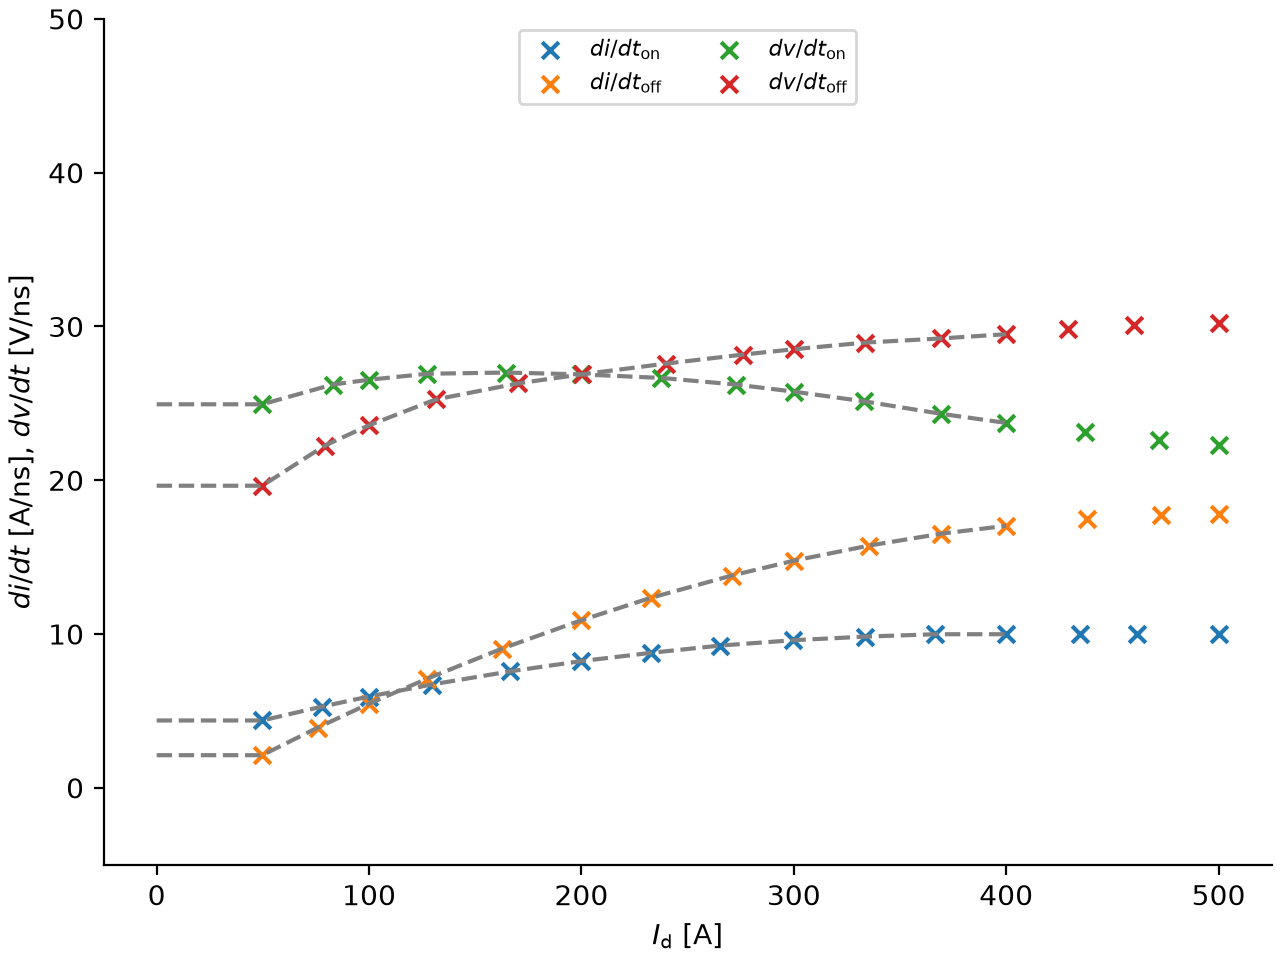
\includegraphics[width=0.62\linewidth]{figures/inputs/switching_slopes.png}
\caption{Switching slopes of the Wolfspeed EDB005M12TM4 as a function of the device current: datasheet points (crosses) and the linear interpolation used by the code (dashed).}
\label{fig:slopes}
\end{figure}

\paragraph{Temperatures and $\Rds(\Tj)$.} The loss per device, $P_\mathrm{dev}=(P_\mathrm{c}+P_\mathrm{s})/(6N_\mathrm{p,mos})$, flows through the case-to-ambient and junction-to-case thermal resistances in series (steady state):
\begin{equation}
\Tc=T_\mathrm{amb}+P_\mathrm{dev}R_\mathrm{th,ca},\qquad \Tj=\Tc+P_\mathrm{dev}R_\mathrm{th,jc}.
\label{eq:thermal2l}
\end{equation}
The on-resistance depends on $\Tj$. The datasheet curve, normalised to \SI{25}{\celsius}, is fitted by a cubic polynomial $\rho(\Tj)=c_3\Tj^3+c_2\Tj^2+c_1\Tj+c_0$ with $\rho(25)=1$ after normalisation (\code{model.rdson_poly_fun}, \code{fit_rdson.py}; \cref{fig:rdson}), and $\Tj$ is clipped to the data range. Since $\Tj$ itself depends on $P_\mathrm{c}$, the code runs a fixed-point iteration with five steps,
\begin{equation}
\Rds^{(k+1)}=\Rds^{25}\,\rho\big(\Tj^{(k)}\big),\qquad \Rds^{(0)}=\Rds^{25},
\label{eq:rdsiter}
\end{equation}
where $\Tj^{(k)}$ comes from \cref{eq:pc2l,eq:ps2l,eq:thermal2l} with $\Rds^{(k)}$ (\code{model.loss_maps}, \code{cycle_eval.losses_2l}). Points outside the envelope (NaN) use the \SI{25}{\celsius} value.

\begin{figure}[ht]
\centering
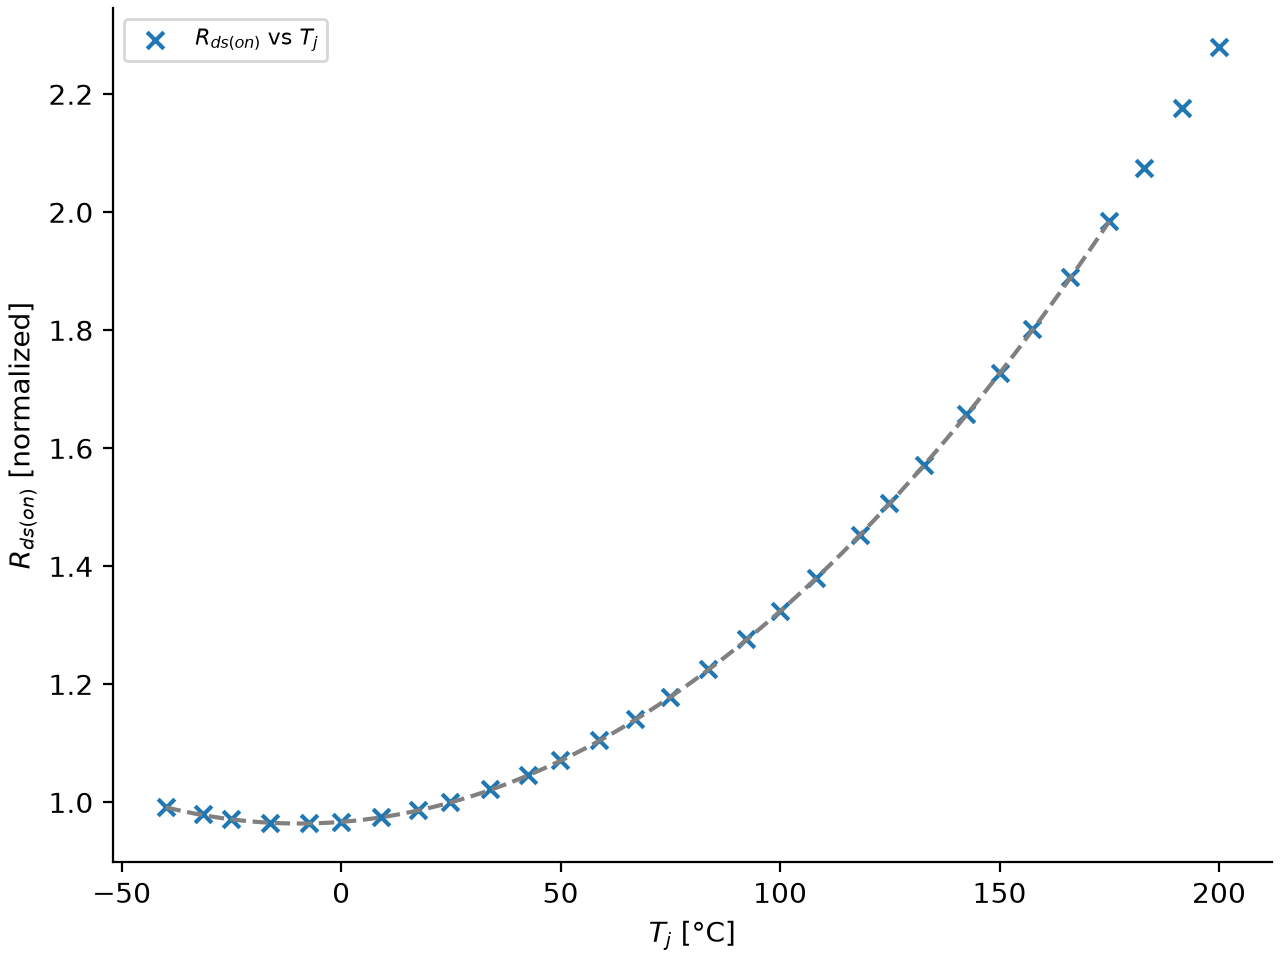
\includegraphics[width=0.48\linewidth]{figures/inputs/Rdson_vs_Tj.png}\hfill
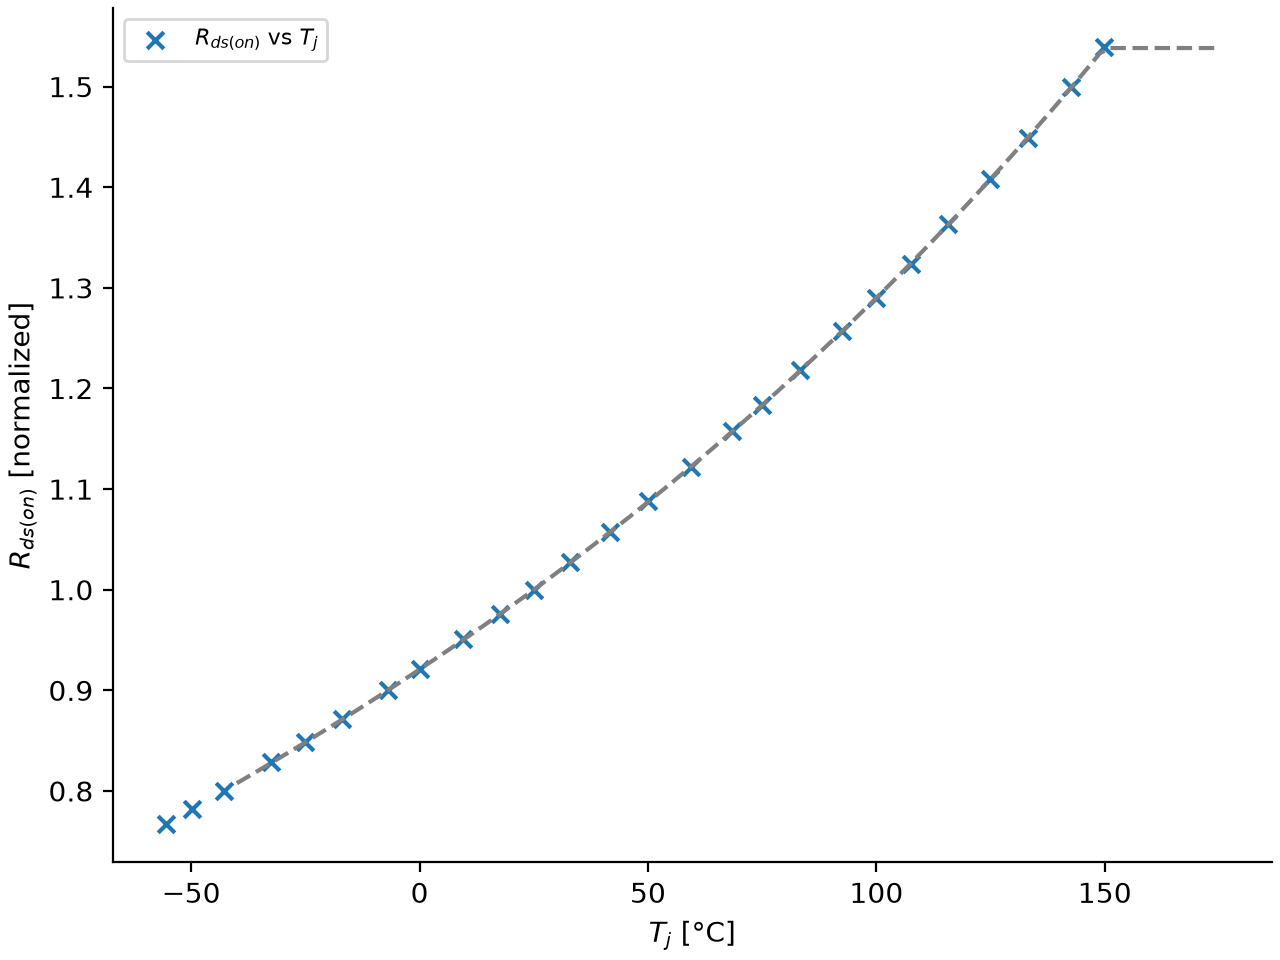
\includegraphics[width=0.48\linewidth]{figures/inputs/Rdson_vs_Tj_bimmc.png}
\caption{Normalised on-resistance versus junction temperature: datasheet points and cubic fit for the 2L SiC module (left) and the Si MOSFET of the BI-MMC (right).}
\label{fig:rdson}
\end{figure}

\paragraph{Battery loss.} The inverter input power is the electrical power of the machine terminals, $P_\mathrm{in}=\tfrac32(v_\mathrm{d}i_\mathrm{d}+v_\mathrm{q}i_\mathrm{q})$, written in the code as $\tfrac32\Ihat\,\hat v\cos(\angle v-\angle i)$. The DC current includes the converter losses, with the sign of the power flow, and the pack loss is the Joule loss in the series and parallel scaled cell resistances (the RC branch is at steady state for a constant current):
\begin{equation}
I_\mathrm{dc}=\frac{P_\mathrm{in}+\operatorname{sgn}(P_\mathrm{in})\,(P_\mathrm{c}+P_\mathrm{s})}{V_\mathrm{dc}(z)},\qquad
P_\mathrm{b}^\mathrm{2L}=I_\mathrm{dc}^2\,(R_0+R_1)\,\frac{N_\mathrm{s}}{N_\mathrm{p}}.
\label{eq:pb2l}
\end{equation}
The DC-link ripple current and the capacitor are not modelled.

\subsection{BI-MMC losses}\label{sec:lossbimmc}
\code{calc.calc_losses_bimmc} has the same inputs and outputs as the 2L function. The converter has $3\Nsm$ SMs with four switches each.

\paragraph{Conduction loss.} In a full-bridge SM the current always flows through two series devices, in the inserted states as well as in the bypass state. The RMS value of a device current is $\Ihat/(\sqrt2N_\mathrm{p,mos})$, so one SM dissipates $2\cdot\tfrac12\Ihat^2\Rds/N_\mathrm{p,mos}$ and the converter
\begin{equation}
P_\mathrm{c}^\mathrm{BI}=3\,\Nsm\,\Rds\,\frac{i_\mathrm{d}^2+i_\mathrm{q}^2}{N_\mathrm{p,mos}}.
\label{eq:pcbimmc}
\end{equation}
It is evaluated with the same fixed-point iteration on $\Rds(\Tj)$ as the 2L drive (\cref{eq:rdsiter}) using the Infineon polynomial.

\paragraph{Switching loss.} The BI-MMC uses the same slope-based scheme, with the SM voltage $v_\mathrm{s}=\Nssm V_\mathrm{cell}(z)$ in place of $V_\mathrm{dc}$ in the voltage intervals of \cref{eq:times}, and constant slopes ($\SI{1}{\ampere\per\nano\second}$ and $\SI{0.5}{\volt\per\nano\second}$ by default). All $4\Nsm$ switches of a phase are assumed to switch once per carrier period, at the frequency $f_\mathrm{c}=m_\mathrm{f}\,p\,\omega_\mathrm{m}/(2\pi)$:
\begin{equation}
E_\mathrm{sw}=\tfrac12v_\mathrm{s}\,\bar\imath\,\big(t_\mathrm{ri}+t_\mathrm{fv}+t_\mathrm{fi}+t_\mathrm{rv}\big),\qquad
P_\mathrm{s}^\mathrm{BI}=3\cdot4\Nsm\,E_\mathrm{sw}\,f_\mathrm{c}.
\label{eq:psbimmc}
\end{equation}

\paragraph{Temperatures.} Analogous to \cref{eq:thermal2l}, with $P_\mathrm{dev}=(P_\mathrm{c}+P_\mathrm{s})/(3\Nsm\cdot4N_\mathrm{p,mos})$ and the thermal resistances of the BI-MMC devices (\SI{0.5}{\kelvin\per\watt} junction-to-case, \SI{0.2}{\kelvin\per\watt} case-to-ambient by default).

\paragraph{Battery loss from the gated phase current.} The cells of an SM carry the phase current while the SM is inserted. For each operating point the code simulates two electrical periods in the time domain with $\theta=\omega_\mathrm{e}t$:
\begin{align}
i_\mathrm{o}(\theta)&=i_\mathrm{d}\cos\theta-i_\mathrm{q}\sin\theta, \label{eq:io}\\
v_\mathrm{ref}(\theta)&=\frac{v_\mathrm{d}\cos\theta-v_\mathrm{q}\sin\theta}{v_\mathrm{s}\,\Nsm\,(1-r)}, \label{eq:vref}\\
g_1&=\big[v_\mathrm{ref}>c(t)\big],\quad g_3=\big[v_\mathrm{ref}<-c(t)\big],\quad s=g_1-g_3\in\{-1,0,1\},\label{eq:gate}\\
i_\mathrm{b}(t)&=g_1\,i_\mathrm{o}-g_3\,i_\mathrm{o}=s(t)\,i_\mathrm{o}(t), \label{eq:ib}
\end{align}
where $c(t)\in[-1,1]$ is a symmetric triangular carrier of frequency $f_\mathrm{c}$ (\code{scipy.signal.sawtooth} with width $0.5$). This is unipolar PWM with a single carrier. All SMs of a phase are assumed to carry the same $s(t)$, so the result of one SM is multiplied by $3\Nsm$. \Cref{fig:pwm} shows one period of these signals. The SM cell string is the equivalent circuit of \cref{sec:sizing}, scaled to $\Nssm$ series and $\Npsm$ parallel cells:
\begin{equation}
R_{0}'=R_0\frac{\Nssm}{\Npsm},\quad R_{1}'=R_1\frac{\Nssm}{\Npsm},\quad C_{1}'=C_1\frac{\Npsm}{\Nssm},
\label{eq:smrc}
\end{equation}
and its state and loss are
\begin{equation}
\frac{\mathrm{d}v_C}{\mathrm{d}t}=\frac{1}{C_1'}\Big(i_\mathrm{b}-\frac{v_C}{R_1'}\Big),\qquad
p_\mathrm{b}(t)=R_0'i_\mathrm{b}^2+\frac{v_C^2}{R_1'}.
\label{eq:rcsim}
\end{equation}
\Cref{eq:rcsim} is integrated with explicit Euler and a step $\Delta t=1/(100f_\mathrm{c})$ (\code{calc.simulate_battery_loss}, compiled with Numba). The first electrical period lets $v_C$ settle and is discarded; the loss is the mean of $p_\mathrm{b}$ over the second period, and the total battery loss is
\begin{equation}
P_\mathrm{b}^\mathrm{BI}=3\,\Nsm\,\big\langle p_\mathrm{b}\big\rangle_{T_\mathrm{e}}.
\label{eq:pbbimmc}
\end{equation}
Explicit Euler with this step is stable only for electrical frequencies above about \SI{8}{\hertz}; the model therefore needs $\omega_\mathrm{e}>0$. On the map grid, the standstill column of the BI-MMC is left empty (NaN); the cycle evaluation applies a speed floor (\cref{sec:cycles}).

\begin{figure}[ht]
\centering
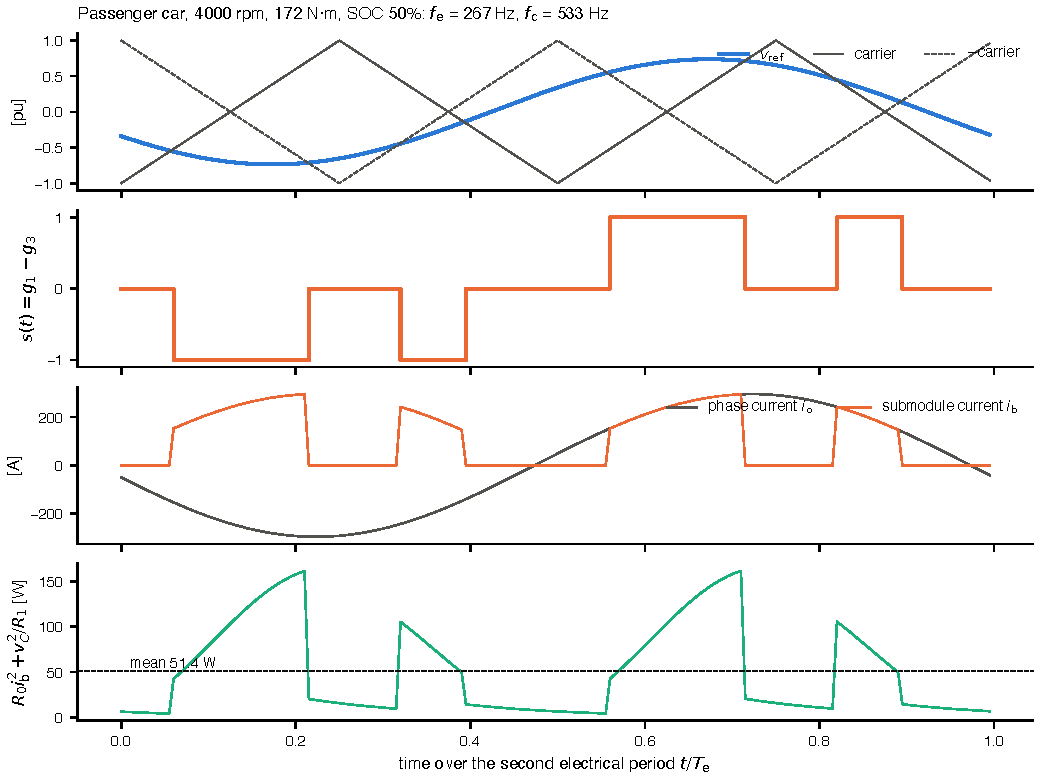
\includegraphics[width=0.85\linewidth]{figures/paper_pwm.pdf}
\caption{BI-MMC battery-loss simulation for one operating point (passenger car): reference and carrier, gating state $s=g_1-g_3$, phase current $i_\mathrm{o}$ and submodule current $i_\mathrm{b}=s\,i_\mathrm{o}$, and instantaneous cell loss. The figure is produced with the equations of the text and checked against \code{calc.simulate_battery_loss}.}
\label{fig:pwm}
\end{figure}

\subsection{Efficiency definitions}\label{sec:effdef}
\paragraph{Operating-point efficiency.} The shaft power is $P_\mathrm{out}=\omega_\mathrm{m}T$, positive in motoring and negative in regeneration, and the total loss is $P_\mathrm{loss}=P_\mathrm{c}+P_\mathrm{s}+P_\mathrm{b}$ (\code{model.efficiency}):
\begin{equation}
\eta=\frac{P_\mathrm{out}}{P_\mathrm{out}+\operatorname{sgn}(P_\mathrm{out})\,P_\mathrm{loss}}.
\label{eq:eta}
\end{equation}
In motoring this is the usual shaft power over input power. In regeneration, \cref{eq:eta} gives $|P_\mathrm{out}|/(|P_\mathrm{out}|+P_\mathrm{loss})$, which stays below \SI{100}{\percent} and equals $1-P_\mathrm{loss}/|P_\mathrm{out}|$ to first order. The efficiency of a single component $k\in\{\mathrm{c},\mathrm{s},\mathrm{b}\}$ is $\eta_k=\eta(P_\mathrm{out},P_k)$. Machine losses are not included.

\paragraph{Cycle efficiency.} For a duty cycle, the efficiency is energy based (\cref{eq:etacyc} in \cref{sec:cycles}).
